\begin{tikzpicture}[x=.5\marginparwidth,y=.5\marginparwidth,>=stealth]
\fill [draw=black,thick,fill=blue!20] (0,0) node [shift={(10pt,4pt)}] {\scriptsize$\theta$} -- (1,0) --(.766,.643) -- cycle;
\draw [dashed,thick] (.766,0)  -- node [pos=.4,left] {\scriptsize$\sin \theta$}(.766,.643);
\draw (.766,5pt) -- ++(5pt,0) -- ++(0,-5pt);
\draw (.5,0) node [below] {\scriptsize$1$};
%\draw [black,dashed] (1,0) arc (0:40:1);
\draw [black,dashed,thick] (1,0) arc(0:40:1) --  (1,.839) -- cycle;
\end{tikzpicture}
% this is the sqrt[x] on [0,5]






